\chapter{Background \& Objectives}
\section{The scenario}
The project is to create a system to produce real time holograms from a camera feed, using the Pepper's Ghost pyramid technique. The system is intended for use at the Aberystwyth Science Week next year, however, there was the potential to display a prototype at the 2017 event held in mid-March. The project is intended to show case a technique, originally used in stage and theatre productions, and give insight into how it can be adapted, with the aid of computer science, to make an impactful visual display.

The system will take real-time data captured from a web cam in the  staging area. The staging area will consist of a black background and appropriate lighting to illuminate the subject. The video feed will then be processed and displayed on a large monitor to work with a ghost pyramid of appropriate size.

To make the final demonstration more interactive, the display will have an accompanying system that allows users to play a charades style game. This would display a topic for the user to act out in the staging area and then allow those viewing the hologram to guess the activity being performed. This would require a system capable of taking multiple different string inputs (guesses) from users simultaneously, and feeding back to all users if a guess is correct. 

\section{Motivation and Justification}
This project is appealing due to the uniqueness of the technology being used to produce it. Whilst the charades game can be considered as a generic system, the creation of real-time holograms is not heavily developed. Many examples of video footage which can be used with the Pepper's Ghost Pyramid are readily available online, however there are far fewer implementations that do real time manipulation for this purpose.

In addition to the project being interesting, it is designed with outreach events in mind therefore giving it value as a potential teaching aide. Pepper's Ghost is an excellent example for children to learn how basic physics and computer science can be used to create an interesting and engaging visual display. In addition, the charades game and real-time hologram system will help to further engage the audience with technique and visualise an impactful application of the technique. 

\section{Background}
\subsection{Pepper's Ghost Pyramid}

The Pepper's Ghost technique was originally used for stage and theatre productions in the Victorian era to display holographic illusions to the audience. The technique, discovered by Dr. Henry Pepper, was first used in theatre in the 1860s\cite{pepper_ghost_comsol} and was used primarily to create a ghost-like illusion.

\begin{figure}[h!]
	\centering{
		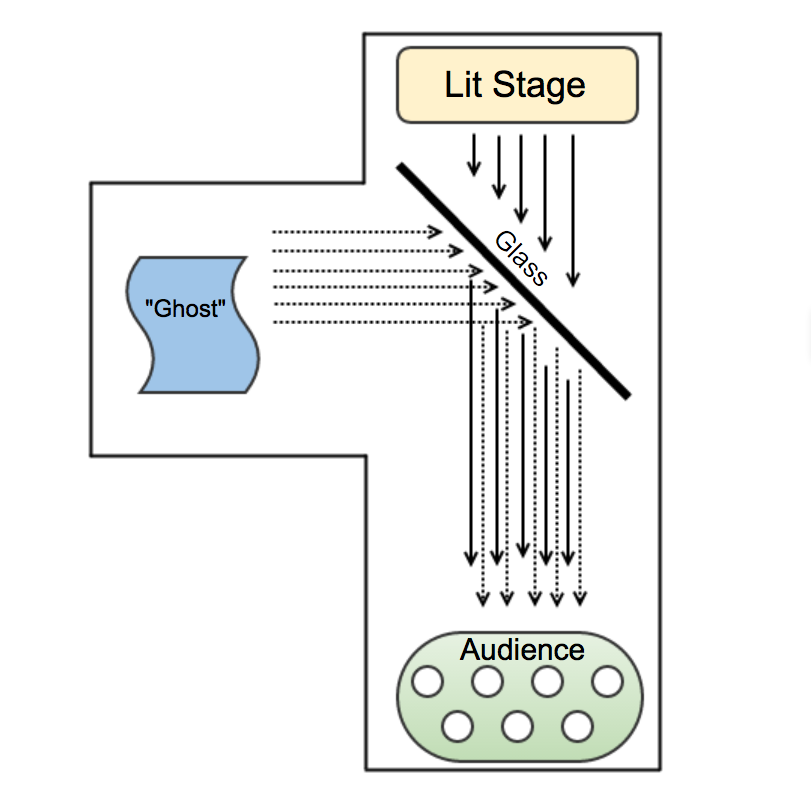
\includegraphics[scale=0.3]{Chapter1/basic_ghost.png}
		\caption{A basic diagram to display the Pepper's Ghost technique's use in theatre. In the diagram solid lines represent light from the lit stage and dashed lines as light from the "Ghost". The image has been taken from Brianne Costa's Blog on the website Comsol \cite{pepper_ghost_comsol}.}
		\label{fig:basic_ghost}
	}
\end{figure}

Figure \ref{fig:basic_ghost} shows a basic example of how the technique produces holographic illusions. The lit stage that is parallel to the viewers line of sight will have actors and scenery as per a normal stage production. The "Ghost" is located off stage and is not visible by the audience. When illuminated, the ghost is displayed to the audience as the light rays travel radially from the "Ghost" and those that reach the glass will be refracted. The glass is positioned at 45\textdegree{} from both the audience and the "Ghost" to account for the 90\textdegree{} offset between the two.

This technique has been modernised since the 1860s, and has been used in different settings proving particularly popular in museums and exhibitions such as \textit{An Audience with Sir Alex Ferguson} at the Manchester United Football Club museum \cite{alex_ferguson} and \textit{Shane Warne - 'Cricket Found Me'} at the national sports museum in Melbourne \cite{shane_warne}.

Within the last few years, there has been a resurgence in the use of the technique with consumers creating there own Pepper's Ghost illusions on mobile devices. Whilst the technique still uses Henry Pepper's original concept, it has been modified to display the hologram from multiple angles using a pyramid - rather than a single glass plane. This structure is commonly referred to as the Pepper's Ghost pyramid.
\begin{figure}[h!]
	\centering{
		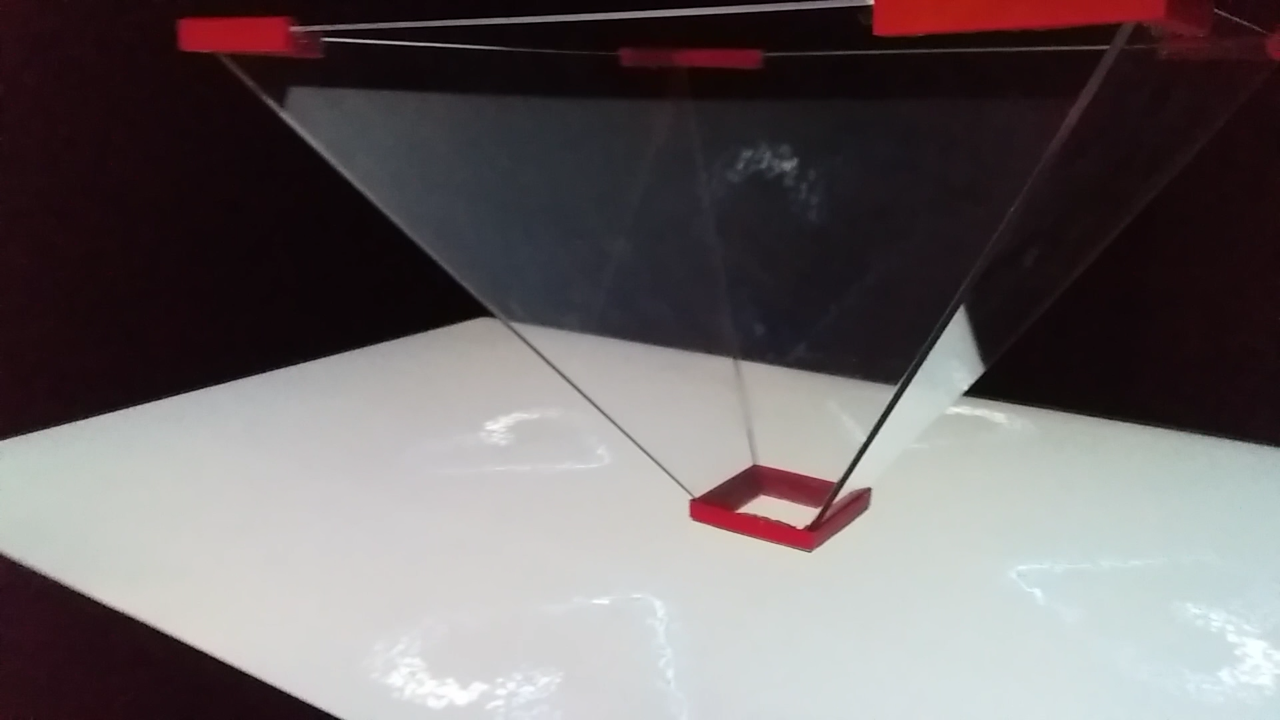
\includegraphics[width=\linewidth]{Chapter1/ghost_pyramid.png}
		\caption{An image of modern day Pepper's Ghost Pyramid made from clear acrylic owned by the Aberystwyth University Computer Science Department.}
		\label{fig:ghost_pramid}
	}
\end{figure}

Figure \ref{fig:ghost_pramid} shows an example of a Pepper's Ghost pyramid. The pyramid is square based, made from a transparent material (such as perspex, clear acrylic or glass) and is open at both the top and bottom. The technique for displaying holograms differs with the "Ghost" now being an image or video displayed on a screen. The pyramid is located on a large horizontal monitor that is being used to display the hologram input images. Furthermore, to create an illusion from all sides of the pyramid, four images are required (one for each side of the pyramid). This  means that the 2D projection of the image can be seen from any side of the pyramid. This Pyramid structure will be used for the hologram creation part of this project.

\section{Analysis}
Whilst there have been numerous examples of applications using the Pepper's Ghost Pyramid as a computer visualisation technique, very few implementation use real time video feeds. This year, 2017, in the presidential election campaign in France, candidate Jean-Luc Melenchon utilised the Pepper's Ghost technique to give a speech to prospective voters in six cities simultaneously \cite{french_elections}. Whilst no precise details of how this system works have been released, this project draws several parallels with the system. Both use the Pepper's Ghost technique with real-time video and therefore this example can be used as a feasibility case for this project. Furthermore, this highlights additional use cases in media and visual representation proving the technique to be of more use than simply an educational tool.

Whilst many have used the technique in an educational setting (such as museums and exhibitions), it is more often the case that the content of the hologram is used as an educational aid, rather than focusing on the technique itself. Due to its simplicity and visual impact, the Pepper's Ghost technique is ideal to help younger children understand light and refraction.  

\subsection{Objectives}
Initially, the project scope covered the creation of a system to produce real-time holograms using a video feed. However, considering the time-line of the project and the work involved, the addition of an accompanying system for the Charades game was added to the objectives. The objectives that were agreed upon are as follows:

\begin{itemize}
	\item To produce a system that can be used for outreach events to show case the creation of holograms using the Pepper's Ghost Pyramid.
	
	\item The system should use real-time video to capture a member of the audience and then project these images as holograms using the Pepper's Ghost Technique.
	
	\item An accompanying system should be produced to allow for a charades style game to be played using the hologram system to display the actor to the viewers.
	
	\item Given the target audience, the system should be interactive and engaging whilst also enabling the viewers to learn about the technique and how it works.
	
	\item The system should be easy to use and for the most part self explanatory.
	
	\item As it is designed for use at outreach events, the system should be robust and thoroughly tested.
	
	\item The system should be easy to run from the perspective of the client. Initial set up should ideally be straight forward and self explanatory.
\end{itemize}


\subsection{Problem decomposition}
Following the agreement of the project objectives, it was possible to begin to decompose the requirements of the project into smaller sections. As the project is comprised of two systems (the real-time Pepper's Ghost creation system and the charades game), this seemed a natural divide for the project at the highest abstraction layer.

\subsubsection{Real-time Pepper's Ghost}
Following research into the Pepper's Ghost technique, it was decided that it would be feasible to construct a prototype of the hologram system for the 2017 Aberystwyth University Science Week event. The main tasks to produce the prototype system were:

\begin{itemize}
	\item Analyse and produce a design for the display area (where the pyramid and monitor are used to produce a hologram).
	
	\item Analyse and produce a design for the staging area (where the actor is filmed).
	
	\item Design and implement a program capable of obtaining a live video feed from a web cam.
	
	\item Correctly orientate and position multiple copies of the video feed in a single display window.

	\item Scale the video feed so it is of the correct size for the output device.

\end{itemize}

The main consideration throughout the development process of the Pepper's Ghost application is the efficiency of the video feed manipulation. To have an effective display, the video should be running at no less than 30 frames per second. An ideal target would be 60 frames a second but this may not be achievable depending on the capture speed of the camera.
 
\subsubsection{Charades game}
The charades game forms the more interactive side of the project. The concept is to have a single actor (member of the audience) outside the viewing area with a mobile device. He or she selects a phrase from a choice of phrases and then acts out the selected phrase. The acting is captured by the web cam from Pepper's Ghost system and displayed as a hologram in the viewing area. Whilst the phrase is being acted, the viewers (who will also have mobile devices) are given information about the phrase (such as the number of words and the genre of the phrase) and attempt to guess what is being acted. Once the phrase has been successfully acted, the actor is be prompted to select a new phrase and the viewers are allocated points. After three phrases, the winner is the viewer with the most points. The main tasks of the charades game are:

\begin{itemize}
	\item Create a user interface for both the actor and viewer.

	\item Allow the actor to select a phrase and, if the phrase is comprised of multiple words, a current word to act.

	\item Allow the viewer to attempt to guess the current word or phrase.

	\item Inform both users when the word or phrase has been correctly guessed.

	\item Prompt the actor for a new word or phrase for them to act.

	\item Establish and implement how and when the game ends.

	\item Inform users of the winner.

	\item Create a session system to only allow those who have logged on to the website with the correct details to access the information.

\end{itemize}

Whilst a mobile application seems ideal for use at localised events, a web app implementation would allow users to access the system from their own mobile devices regardless of platform. However, using a web app raises additional security issues that should be taken into consideration. To stop malicious interactions from those outside the event, the web app must ensure that only those at the event can access the system. To ensure this, the main task list included adding a session key to the system. This session key will be distributed at the event, and only those who know the session key are able to access the system. The system also provides the ability to change the session key easily when required.

\subsection{Alternative implementations}
Implementing an android application boasts increased security as devices could potentially connect via Bluetooth or a peer-to-peer connection. The shorter connection range offered by these technologies, would mean that those outside the event would not be able to join session and corrupt the system. Furthermore, it would stop users from attempting to change the information in the URL for each page and therefore reduce the number of checks required to ensure that the system data has not been tainted.

Despite this, a web application done correctly is more accessible to users as it is platform independent. In addition, it would be possible for users to access the system from their own devices, such as smart phones, meaning more users can play the game at the same time.

\section{Process}
After consideration of different methodologies, the decision was made that this project would follow the Feature Driven Development (FDD) plan driven methodology. FDD is normally considered for larger projects as it provides a framework for distributed development. By dividing developers into smaller teams, FDD allows those teams to tackle features one at a time in parallel. Furthermore, the up front planning stage is generally more suited to projects that are more stable as, whilst it can be adapted throughout the process, the overall model is normally only added to, and the core architecture remains static. FDD follows five steps throughout the development of a software system. The first three steps regarding planning and designing an overall model, and developing a list of all the features that must be considered for the system to meet the criteria of the end users. The remaining two step form an iterative process of designing and implementing features one by one.

The steps required to complete this project are well defined and therefore would be well suited to having an up front design. Furthermore, FDD encourages continuous integration (CI) which offered a way to produce a functional prototype at various stages of the project. CI was a significant aid for producing a function prototype for both the mid project review and the 2017 Aberystwyth University science week event. FDDs \textbf{Design by feature} stage offers an ideal step to perform spike work for technologies that are unfamiliar to the developers. Moreover, it was still possible to follow the five step process of FDD development in this project.

\subsection{Single Person FDD adaptation}
To successfully use FDD for this project, several adaptations to the normal processes of the methodology were made. Many of these changes mirror those discussed in S. Khramthchenko's thesis, \textit{"A Project Management Application for Feature Driven Development (FDDPMA)"} \cite{single_person_fdd}. The most notable being the abolition of developer teams in favour of a single developer. This required the developer to assume multiple roles throughout the development process and at each different stage as specified below.

\subsubsection{Develop an Overall Model}
Initially, a Domain Expert (Customer) was required to aid in the development of the overall model and feature creation. In this context, the project supervisor (Dr. Helen Miles) fulfilled this role and the developer acted as both the Chief Programmer and Chief Architect. For this project, the Domain specific language was shared by both the Domain Expert and the developer.

\subsubsection{Build a Feature list}
The feature list was produced with the objectives of the system and  the main tasks for the project in mind. This was finalised with a discussion between the developer and the Domain Expert which verified all the features. In addition to a description, each feature also had a complexity and priority rating, as well as a list of dependent features and whether the feature was require for the prototype. The final feature list is shown in Figure \ref{fig:feature_list}.

\begin{figure}[h!]
	\centering{
		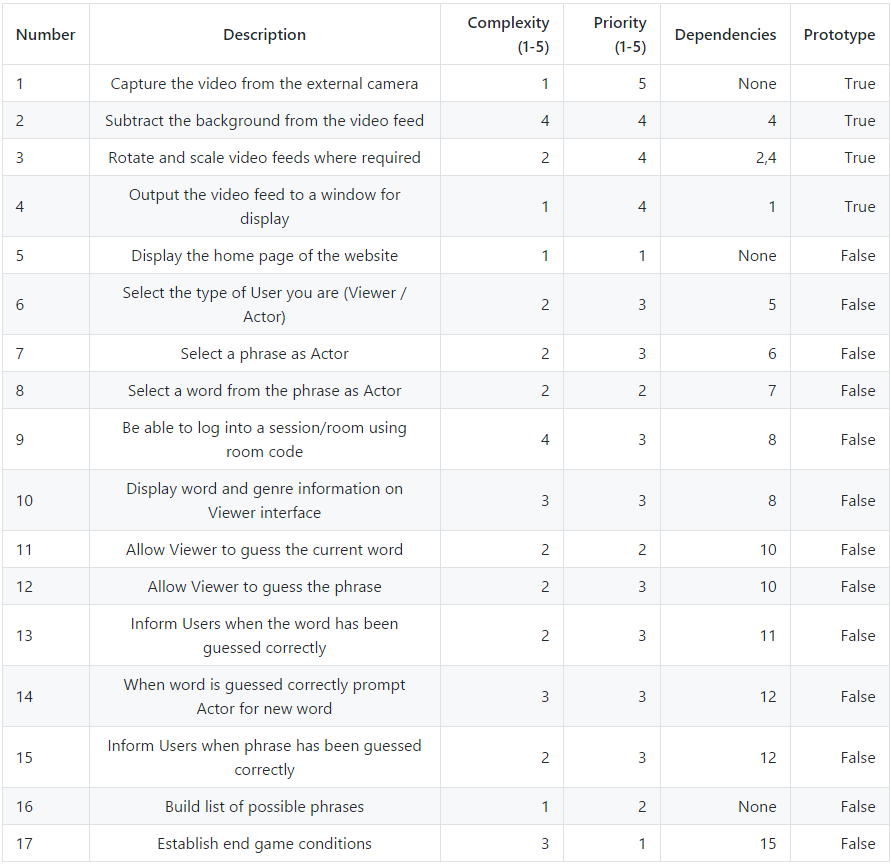
\includegraphics[width=\linewidth]{Chapter1/feature_list.png}
		\caption{The full feature list for the project }
		\label{fig:feature_list}
	}
\end{figure}

\subsubsection{Plan by Feature}
Steps such as establishing developer teams and scheduling developer teams' time throughout the project were no longer required. In their place, the features were given priorities to aid time scheduling and development order. Once the order was created, the features were assigned to separate week long iterations.

\subsubsection{Design by Feature}
Features were selected in dependency order. Once selected, features were exhaustively designed taking into consideration the functions required to fulfil the feature as well as how these functions should be tested. The project used GitHub for version control and issues were created which corresponded to a feature. The first action in an issue was to complete a design of the feature and update the overall design as required.

\subsubsection{Implement by Feature}
Features were implemented in the same GitHub issue as the design work. The project was developed using Test Driven Development (TDD) and, therefore, the test suite was updated before any code was implemented. Once the tests were created, an implementation was added which had to pass the tests to be acceptable. Whilst the tests could be run locally, there was also a Jenkins service for continuous integration to run the full test suite before it was merged with the master branch.  
